\documentclass[a4paper]{article}

\usepackage{listings}
\usepackage{xcolor}
\usepackage{hyperref}
\usepackage{graphicx}
\usepackage{geometry}
\usepackage{algorithm}
\usepackage[noend]{algpseudocode}
\usepackage{amsmath}
\geometry{margin=1.5in}
\usepackage[english]{babel}
\usepackage{url}
\usepackage{titling}

\setlength{\droptitle}{-11em}

\title{EnGPar - Partitioning and Load Balancing for Relation Based Data}

\author{Gerrett Diamond}

\date{\today}

\begin{document}

\maketitle

\section{Introduction}
A main problem in parallel applications is ensuring a even distribution of load across all the processors. While some applications can naively distribute data evenly, many applications have complicated designs that require load balancing procedures that partition in order to minimize both the computation and communication costs. For finite element programs that utilize unstructured meshes, there exists a complicated structure of computation and communicative costs that depend on where degrees of freedoms are defined and the type of shape functions being used. Thus any load balancing technique must offer a diverse set of procedures to target the different levels of imbalance relative to the finite element method being applied. To target the different load balancing requirements we propose utilizing an expanded graph structure, N-graph \cite{EnGPar2015proposal}, that can represent multiple levels of relations simultaneously coupled with a set of partitioning techniques and diffusive load balancing strategies.
This paper provides an overview of the N-graph structure and the framework for diffusive load balancing in EnGPar. Some examples of partitioning strategies are given in section 2. Section 3 describes the details of the N-graph structure and some components needed for use in diffusive load balancing. Then the framework and some details on diffusive load balancing is given in Section 4. Section 5 and 6 provide an experiment of the diffusive load balancing technique. Finally, Section 7 discusses some further work in this topic to be explored.

\section{Related Works}
\subsection{Geometric Partitioning}
Some of the fastest and simplest partitioning techniques are geometric partitioning algorithms that utilize coordinate information on the data and partition just based on the spatial distribution of the data. Some of these techniques include Recursive Coordinate Bisection and Recursive Inertial Bisection \cite{chevalier2012load,TaylorRIB,williamsRIB} which recursively partition the data by defining cut planes in space to create the parts. While these techniques are relatively fast and can partition the data well, the edge cut across parts is often poor and thus the communication costs tends to be quite high. Furthermore, there is no consideration given to multi-criteria partitioning for these techniques so there is no guarantee that the partitioning will be sufficient for finite element methods.

\subsection{Graph Partitioning}
The most common methods to partition relation-based data structures is utilizing a graph or hypergraph structure to represent the data followed by partitioning techniques that are performed on the structure. Some commonly used libraries to perform graph partitioning include ParMETIS \cite{parmetis4} and PT-Scotch \cite{scotch2009}. These algorithms globally partition the data targeting balancing the vertices of the graph in each part and the edge cut across parts. These algorithms tend to work well for simple relation structures but can fail when there are multiple criteria to be balanced simultaneously. For example when partitioning unstructured meshes, graph partitioning tends to have high mesh vertex imbalances which can be detrimental for finite element procedures that have degrees of freedom on the mesh vertices. 

On top of graph partitioners there are also hypergraph partitioners that utilize hyperedges to better represent the communication costs between processors for highly interconnected relation-based data structures like unstructured meshes \cite{devine2002zoltan}. These techniques tend to decrease the overall edge cut and reduce the communication volume across parts. Like graph partitioning, hypergraph partitioning also suffer from having high imbalances of any entities in the data that are not represented as graph vertices. 

\subsection{Diffusive Load Balancing}
Typically less powerful but faster than graph partitioning techniques are diffusive load balancing methods which iteratively migrate data from high load parts to the lower loaded neighbors across part boundaries. These methods like ParMA \cite{SmithParma2015} allow techniques that can target different metrics as well as multiple criteria simultaneously which other methods cannot. These methods are often used as a routine to improve upon a partition as the migrations are only done locally between a part and its neighbors instead of the global partitioning seen in geometric and graph partitioning techniques.

\section{Ngraph}
EnGPar interfaces to the different partitioning procedures through a graph abstraction called the N-graph. Towards supporting a combination of (hyper)graph, geometric and diffusive partitioning methods on relation-based data, the N-graph is defined as $G^n(V,E_0,E_1,...,E_{n-1},[P_0,P_1,...,P_{n-1}])$ where:
\begin{itemize}
  \item $V$ atomic units $u_i$ of the domain $\omega$ which uniquely exist on one
    part such that $\omega = \bigcup_{\forall_i}u_i$, and 
  \item $E_i$ relations $e_i$ of type $i$ that represent either a traditional edge between two vertices, $u$ and $v$, or a hyperedge which relate a set of vertices
  \item $P_i(e,v)$ pins in the case of hyperedges which represent the connection
    from $e$ to $v$ where $e \in E_i$ and $v \in V$.
\end{itemize}
Optionally, the vertices and edges may be assigned with weights to better control partitioning. Vertices may also have spacial relations in the form of a coordinate vector $c$.

\begin{figure}[!ht]
  \centering
  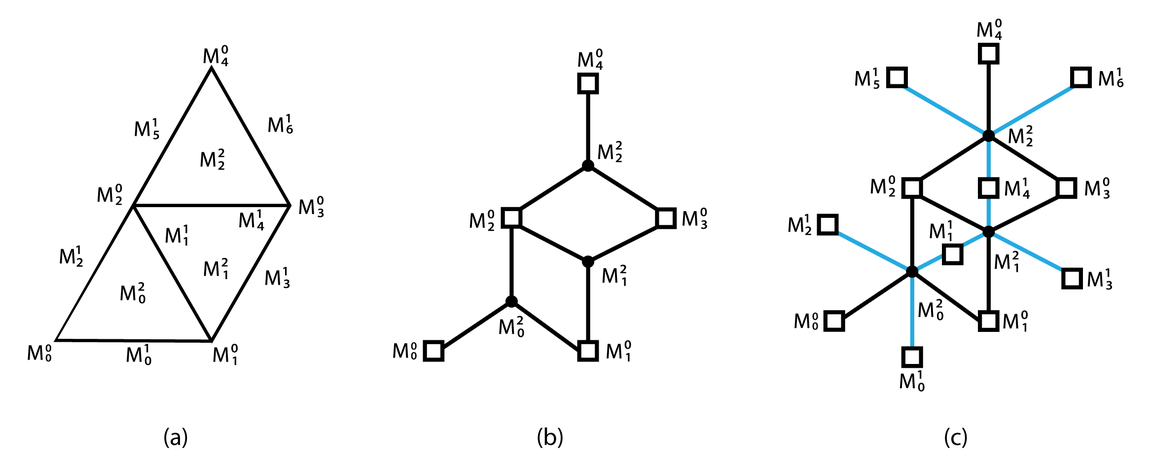
\includegraphics[width=\textwidth]{exampleMesh2Graph.png}
  \caption{(a) a 2D unstructured mesh. (b) Ngraph construction with elements$\rightarrow$vertices, vertices$\rightarrow$hyperedges. (c) Additionally edges$\rightarrow$second hyperedge}
  \label{fig:Mesh2Graph}
\end{figure}

Applications utilizing this abstraction define atomic domain entities as vertices in the N-graph and at least one relation between them as the (hyper)edges. In this manner, applications may represent multiple relations of different sparsity and degree. For example the topology of an unstructured 3D mesh may be represented via vertices defined as mesh elements and a hyperedge type for each entity shared by adjacent elements. Figure \ref{fig:Mesh2Graph} depicts the mapping of an unstructured mesh (a) to a representation where mesh elements map to graph vertices and mesh vertices map to graph hyperedges (b) and a second mapping where mesh edges are mapped to a second edge type in the graph (c).

\subsection{Migration}
In order to support diffusive load balancing, an internal migration procedure is required to allow iterative changes of the data structure. Having to perform several small migrations constantly introduces a challenge in how to construct the data structure optimally to allow quick changes.

One solution to this problem, as seen in PUMI for use in ParMA \cite{ibanez2016pumi}, is to allocate extra storage where necessary in order to allow easy inserts and deletes into the data structure without having to restructure entire portions of it. This results in a migration procedure which runs in time proportional to the number of entities being migrated. While this method is fast it has a memory concern on having this extra storage. On top of that there is the question of how large the extra storage needs to be to ensure it never overflows. For the case of PUMI, the data structure is a mesh and adjacencies are mostly limited due to spatial considerations. For general graphs, especially those seen in real world networks, there is no limitation on the number of adjacencies and defining some large constant to support real world networks where only a few vertices have very high degree would be a large waste of memory. To further motivate against this strategy is that when expanding to data parallel architectures like GP-GPUs this method is not well suited.

An alternative approach, focusing on data parallel techniques, is for each migration the entire data structure is reformatted to compactly store the new set of adjacencies. This approach comes with a penalty where each migration no matter the size must perform a total reconstruction of the graph which means the runtime is proportional to the number of vertices and edges on part. However the data is always compactly stored for the amount that is currently on process. We use this approach for migration due to its natural data parallel design. Algorithm \ref{alg:migration} details psuedocode for the implementation of this approach in EnGPar.
\newpage

\begin{algorithm}
\caption{Migration}\label{alg:migration}
\begin{algorithmic}
  \Procedure{migrate}{plan}
  \State updateGhostOwners(plan)
  \For {each local vtx}
  \If {vtx is not in plan}
  \State local\_verts$\leftarrow$ vtx
  \For {each edge of vtx}
  \If {edge is not added}
  \State local\_edge $\leftarrow$ edge
  \EndIf
  \For {each pin of edge}
  \If {this part does not own pin}
  \State ghost\_verts $\leftarrow$ pin
  \EndIf
  \EndFor
  \EndFor
  \EndIf
  \EndFor
  \For {each vtx in plan}
  \For {each edge of vtx}
  \State affectedEdges $\leftarrow$ edge
  \EndFor
  \EndFor
  \For {each vtx in plan}
  \State send vtx to new owner
  \EndFor
  \For {each received vtx}
  \State local\_verts$\leftarrow$ vtx
  \EndFor
  \For {each edge in affectedEdges}
  \State residence = getResidence(edge)
  \For {each part in residence}
  \State send edge to part
  \EndFor
  \EndFor
  \For {each received edge}
  \State local\_edge$\leftarrow$edge
  \For {each pin of edge}
  \If {this part does not own pin}
  \State ghost\_verts $\leftarrow$ pin
  \EndIf
  \EndFor
  \EndFor
  reconstructGraph(local\_verts,local\_edges,ghost\_verts)
  \EndProcedure
  
\end{algorithmic}
\end{algorithm}

\section{Diffusive Load Balancing}
\subsection{General Framework}
In order to support continuously new methods of diffusive load balancing and new criteria and priorities, a general algorithm is defined for both ease of use and creation for future use of EnGPar. Algorithm \ref{alg:balancer} lists psuedocode for the overall design of the balancer. For each diffusive technique being implemented five methods need to be defined:
\begin{itemize}
  \item $makeSides$\\
    Each process calculates the length of the part boundaries to all neighbors.
  \item $makeVtxWeights$ \\
    Each process calculates the weight of its own vertices and shares with each neighboring process.
  \item $makeEdgeWeights$ \\
    Each process calculates the weight of its own edges and shares with each neighboring process.
  \item $makeTargets$\\
    Each process calculates the amount of weight to send to each of its neighbors.
  \item $makeSelector$\\
    Makes a migration plan of the vertices to send to neighboring processes based on the iteration queue and amount of weight being sent.
\end{itemize}
Further operation control is also possible through changing the $createIterationQueue$ function which controls the order that graph vertices are iterated when selecting for migration. Stagnation detection is utilized to ensure that the balancer ends after no more improvements are found rather than completing any further unproductive iterations.

\begin{algorithm}
\caption{Diffusive balancer design}\label{alg:balancer}
\begin{algorithmic}
  \Procedure{runStep}{Ngraph g}
  \State sides = makeSides(g)
  \State vtxWeights = makeVtxWeights(g,sides)
  \For {each edge type i}
  \State edgeWeights[i] = makeEdgeWeights(g,sides,i)
  \EndFor
  \State targets = makeTargets(g,sides,vtxWeights,edgeWeights)
  \State pq = createIterationQueue(g)
  \State selector = makeSelector(pq)
  \For {increasing cavity size,cavSize}
  \State plan $\leftarrow$ selector.select(targets,cavSize)
  \EndFor
  \State g.migrate(plan)
  \State Update Stagnation Detection
  \EndProcedure
  \Procedure{balance}{Ngraph g}
  \State iter=0
  \For {iter=0 to maxIter}
  \State runstep(g)
  \If {balance has stagnated or g is sufficiently balanced}
  \State return
  \EndIf
  \EndFor
  \EndProcedure
\end{algorithmic}
\end{algorithm}

\subsection{Vertex Balancer}
As proof of concept a simple diffusive vertex balancer was implemented off of this design. The vertex balancer targets balancing the sum of the weights of the vertices in the graph. To do so we implement the five basic functions mentioned previously as follows. The $makeSides$ function has each part compute $s_i$ which is the number of (hyper)edges that are cut between this part and part $i$. This way each part knows which parts are its neighbors and has a metric representing the length of the boundary to the part. Second is the $makeVtxWeights$ function. This function has each part compute the sum of the weights of the local vertices and shares this value with each of its neighbors. Thus each part has a weight, $w_i$, that corresponds to each $s_i>0$. The $makeEdgeWeights$ function does nothing for this balancer since it only prioritizes the vertex weight. The $makeTargets$ function takes each neighboring weight and if the part's weight is greater than the neighbor's weight than it computes the amount of weight to send to that part in this iteration. This value is equal to 
$$(w-w_i)*\dfrac{s_i}{\sum{s_i}}*\text{factor}$$
where the factor is some parameter that controls the step size of each iteration. The final piece, $makeSelector$, is a selection procedure that traverses the given iteration queue and selects cavities that are shared between a part and a target neighboring part. For now the selector is kept simple for testing cases, but in future iterations will include capabilities such as canceling some parts of the migration plan to account for multi-criteria or improving some metric for specific load balancing goals.

\subsection{Extending to Multi-Criteria Balancing}
In order to advance to multi-criteria load balancing we have to expand some of the functionality created in the vertex balancer. The $makeSides$ and $makeVtxWeights$ functions will be unchanged since they act similarly. However now the $makeEdgeWeights$ function will be used to calculate the weights of each edge type that is being targeted. The $makeTarget$ function will have to be altered to take into account the edge weights given by the $makeEdgeWeights$ function as well as look at the priorities of the edge types and vertices given by the user. The biggest change required is to the selector which has to take into account the weights of all edge types being balanced and make appropriate changes to the migration plan to ensure that the partition improves in each iteration. 

\section{Experiments}
A set of test cases were run on balancing a prepartitioned 3D unstructured mesh were run to compare EnGPar's graph vertex balancer to ParMA's mesh element balancer. The tests were run on a torus mesh split into four parts with four levels of refinement. The meshes were approximately 16, 42, 126, and 391 thousand elements where each element was given the same weight of one. Each mesh is partitioned such that two parts have a much higher load than the other two parts resulting in an imbalance of roughly 46\%. Figure \ref{fig:torus} shows the initial partitioning of the 391 thousand element mesh colored by part number. Each mesh is run with both ParMA and EnGPar using the vertex balancer with the weight factor$=0.1$. Each case runs some amount of iterations until the imbalance has converged to some value below 10\%.


\begin{figure}[!ht]
  \centering
  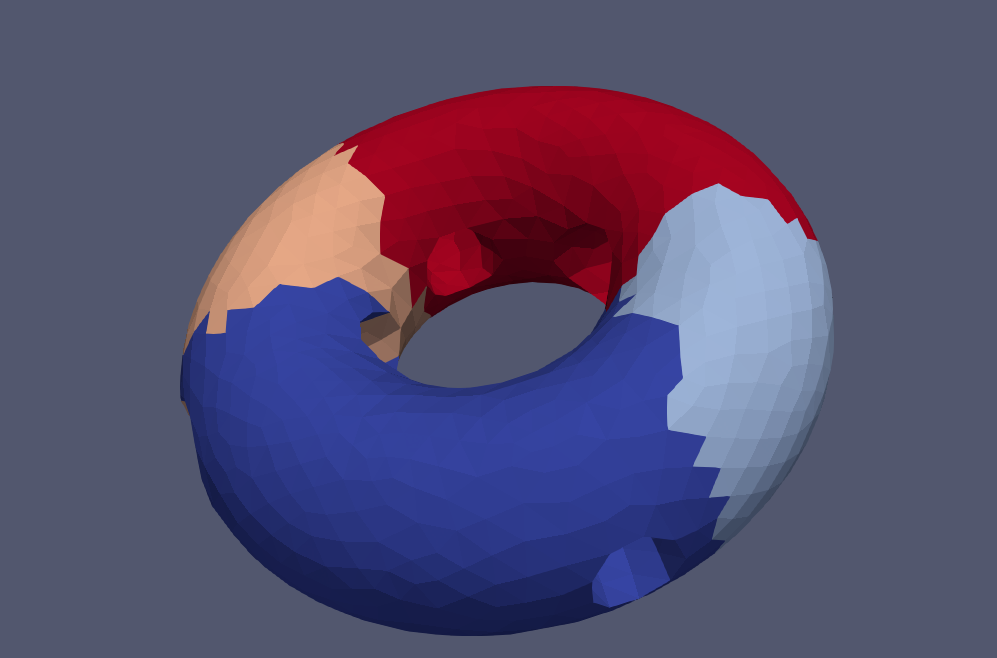
\includegraphics[width=250px]{torus.png}
  \caption{Four part torus mesh with two highly loaded parts}
  \label{fig:torus}
\end{figure}


\section{Results}
For each mesh, two metrics are recorded for both ParMA and EnGPar. The first is the number of iterations it takes to converge and the second is the total time until convergence. The iterations of each run can be found in Table \ref{tbl:iterations} and the runtimes can be found in Figure \ref{fig:runtime}. The first thing to note is that EnGPar takes a few more iterations for each case to converge than ParMA. This is a result of a limitation on the current iteration queue and selector which limits the amount of vertices that can be sent in a given iteration to those vertices on the part boundary. While this does result in more iterations as one can see the time it takes for EnGPar to converge is still smaller than ParMA in all four runs. This leads hope that fixing the limitation on the weight being sent in each iteration and converging in less iterations will result in larger speed improvements. Further concept on this improvement is that approximately 90\% of an iteration in EnGPar is performing migration on the mesh. Since the time of migration is largely based on the size of the mesh, performing larger migrations less frequently should see major improvements to the runtime of EnGPar. After removing the limitation, efforts will have to go into defining what an appropriate value of the weight factor should be in order to get a more optimal balance between sending large enough migrations and not over sending weight that it takes longer to converge and thus more migrations needed.

\begin{table}
  \centering
  \begin{tabular}{|c|c|c|}
    \hline
    Num of elements & EnGPar & ParMA \\
    (thousand) & & \\
    \hline
    16 & 15 & 8 \\
    42 & 10 & 9 \\
    126 & 12 & 10 \\
    391 & 16 & 13 \\
    \hline
  \end{tabular}
  \caption{Number of iterations to converge to 10\% imbalance}
  \label{tbl:iterations}
\end{table}

\begin{figure}[!ht]
  \centering
  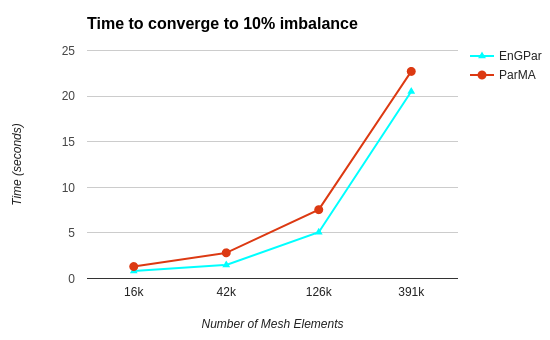
\includegraphics[width=300px]{timeTorus.png}
  \caption{Runtimes for EnGPar and ParMA balancing a four part torus mesh.}
  \label{fig:runtime}
\end{figure}

\section{Future Work}
As detailed earlier, for multi-criteria load balancing there is much work to be done to add functionality to the selector in order to properly balance the range of priorities any given user could have. Continuing on that the selector will need to have the ability to correct the plan by canceling portions of the migration plan to best balance based on the different criteria.

Another portion that can have a major impact on the quality of partitioning for these diffusive methods is the order in which the vertices are iterated over. The current method is iterating blindly over how the vertices are stored in memory with no regards to the overall structure of the part. While this will result in balancing the vertices, for some instances the parts can become elongated and result in large diameters. In ParMA \cite{SmithParma2015}, the iteration follows a graph distance based metric which prioritizes mesh elements that are further away from the part centroid. This method results in rounder parts and smoother part boundaries as well as reducing the diameter of the part. Further work will go into implementing this method into EnGPar and also exploring other options and what metrics are effected by the order of iteration.

\section{Closing Remarks}
Diffusive load balancing techniques offer a fast way to iteratively improve the partition of a relation based structure through the ability to use different sets of metrics to define the different layers of load in the structure. EnGPar along with the N-graph structure provide a light-weight interface that allow faster and easier usage of techniques shown to work on specific structures such as ParMA for load balancing unstructured meshes. In this paper, we discussed the beginning work for diffusive load balancing methods being used on the N-graph as well as methods to advance the techniques to the levels seen in the current methods being used.


\newpage \bibliographystyle{plain}
\bibliography{scorec-refs/scorec-refs}

\end{document}
